\begin{notation}[\cite{endrullis2024generalized}] For morphisms \( \alpha : A \to B \), \( \beta : B \to C \), \( \gamma : A \to C \) and $E \subseteq \operatorname{Hom}(A,B)$, define:
 \begin{flalign*}
            \set{ \alpha \star - = \gamma } &\overset{\operatorname{def}}{=} \{ \beta \in \operatorname{Hom}(B, C) \mid \alpha \star \beta = \gamma \}.
\\
            \set{ - \star \beta = \gamma }  &\overset{\operatorname{def}}{=} \{ \alpha \in \operatorname{Hom}(A, B) \mid \alpha \star \beta = \gamma \}.
\\
            E \star \beta                   &\overset{\operatorname{def}}{=} \set{ \alpha \star \beta \mid \alpha \in E }.
 \end{flalign*}
\end{notation} 

\begin{definition} 
    \label{def:bigodot}
Let $(S, \oplus, \odot, 0_s, 1_s)$ be a semiring. We define 
 \begin{flalign*}
    \bigodot \emptyset &\overset{\operatorname{def}}{=} 1_s
\\
    \bigodot \left( E \cup \{x\} \right) &\overset{\operatorname{def}}{=} \left( \bigodot E \right) \odot x
    \\
    \bigoplus \emptyset &\overset{\operatorname{def}}{=} 0_s
    \\
        \bigoplus \left( E \cup \{x\} \right) &\overset{\operatorname{def}}{=} \left( \bigoplus E \right) \oplus x
\end{flalign*}
\end{definition}


\begin{definition}[Morphism weight \cite{endrullis2024generalized}]
    \label{def:weight}
    Let $\mathcal{T} = (T,\mathbb{E},S, w)$ be a finitary type graph.
    \newline
    \noindent
    \begin{minipage}{0.6\textwidth}
        The \textbf{weight of a morphism $h: G \rightarrow T$ relative to $(e:X \to T) \in \mathbb{E}$} is defined as the weight $w(e)$ raised to the power of the number of $\iota$ making the diagram (shown on the right) commutative.
    \end{minipage}
    \begin{minipage}{0.29\textwidth}
        \begin{center}
                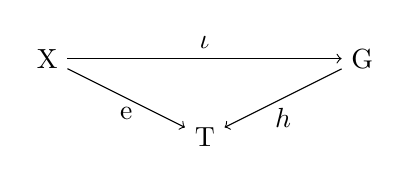
\begin{tikzpicture}
                    \node (a) at (0,0) {X};
                    \node (c) at (4,0) {G};
                    \node (d) at (2,-1) {T};
                    \draw[->] (a) -- (d) node [midway,below] {e};
                    \draw[->] (a) -- (c) node [midway,above] {$\iota$};
                    \draw[->] (c) -- (d) node[midway, below] {$h$};
                    % \node (d) at (2,-0.5) {=};
                \end{tikzpicture}
        \end{center} 
    \end{minipage}
                \[
                w_e(h) 
                    \overset{\operatorname{def}}{=}
                \underset{\alpha \in \{- \star h = e\}}{\bigodot}w(e) 
                \]
        % which can be visualized as $w(e)$ raised to the power of the number of possible morphisms $g$ which make the following commutative diagram hold

        \noindent
        The \textbf{weight of a morphism $h: G \rightarrow T$ relative to \(\mathcal{T}\)} is defined as the semiring product of $w(e)$ for $e \in \mathbb{E}$:
        \[  w_\mathcal{T}(h) \overset{\operatorname{def}}{=} \underset{e \in \mathbb{E}}{\bigodot} 
                w_e(h) \]

        \noindent
       The \textbf{weight of an object \( G \in \mathcal{C}_0 \) relative to \( \mathcal{T}\)} is defined as the semiring sum of $w_\mathcal{T}(h)$ for $h \in \operatorname{Hom}(G,T)$:
        \[w_\mathcal{T}(G) \overset{\operatorname{def}}{=} \underset{h \in \operatorname{Hom}(G,T)}{\bigoplus}  w_\mathcal{T}(h) \]
\end{definition}


% In certain scenarios, we want to exclude specific morphisms when calculating morphism weight relative to a give T-valued element $e:X \to T$. For this reason, for all set \( \Gamma \subseteq \operatorname{Hom}(A, G) \), we define 



% The weight of the morphism \( \phi : G \to T\) excluding morphisms in \( \Gamma' \) is defined as the number of morphisms from \( X \) to \( G \) that do not factor through any \( \alpha \in \Gamma \).
\todo{This starts to be quite hard to follow without intuition or example}
\begin{definition}[Weight excluding specific morphisms \cite{endrullis2024generalized}]
    \label{def:weight_excluding}
    Let \( A \in \mathcal{C}_0 \) and $\Gamma \subseteq \operatorname{Hom}(A,G)$.
    \newline
    \noindent
    \begin{minipage}{0.6\textwidth}
        We define $\Gamma'$ as the set consisting of all morphisms \( \iota : X \to G \) admitting morphisms \( \zeta \colon X \to A \) and \( \alpha \in \Gamma \) such that the diagram illustrated on the right is commutative. Formally, 
    \end{minipage}
    \begin{minipage}{0.4\textwidth}
        \hfill 
        % \begin{center}
            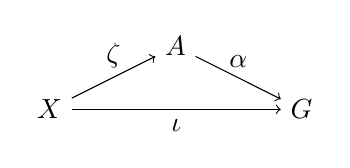
\begin{tikzpicture}[scale=0.8]
                \node (X) at (0,0) {\(X \)};
                \node (A) at (2,1) {\( A \)};
                \node (G) at (4,0) {\( G \)}; 
                \draw[->] (X) -- (A) node[midway, above] {\( \zeta \)};
                \draw[ ->] (X) -- (G) node[midway, below] {\( \iota \)};
                \draw[->] (A) -- (G) node[midway, above] {\( \alpha \)};
                % \node at (2,0.5) {\( = \)};
                % \node (T) at (2,-1) {\( T \)};
                % \draw[ ->] (X) -- (T) node[midway, below] {e};
                % \draw[<-] (T) -- (G) node[midway, above] {};
            \end{tikzpicture}
        % \end{center} 
    \end{minipage}

    \[
    \Gamma' \overset{\operatorname{def}}{=} \left\{ \iota \in \operatorname{Hom}(X, G)~\middle|~\exists \alpha \in \Gamma,~\exists \zeta:X \to A,~\zeta \star \alpha = \iota \right\}.
    \]

    \noindent
    The \textbf{weight of a morphism \(h : G \to T\) excluding morphisms in \( \Gamma' \) relative to $(e:X \to T) \in \mathbb{E}$} is defined as $w(e)$ raised to the power of the number of morphisms \( (\iota : X \to G) \notin \Gamma' \).
        \[
        w_e(h - \Gamma) \overset{\operatorname{def}}{=} \underset{
            \substack{\alpha \in \set{- \star h = e} \\
                        \alpha \notin \Gamma'}}{\bigodot} w(e)\] 
        The \textbf{weight of a morphism $h: G \to T$ excluding morphisms in \( \Gamma' \) relative to \(\mathcal{T}\)} is defined as the semiring product of $w_e(h-\Gamma)$ for $e \in \mathbb{E}$:
        \[ 
            w_\mathcal{T}(h-\Gamma) \overset{\operatorname{def}}{=} \underset{e \in \mathbb{E}}{\bigodot} 
        w_e(h-\Gamma)
                \]
\end{definition} 
% \begin{definition}[Weight excluding morphisms \cite{endrullis2024generalized}]
%     \label{def:weight_excluding}
%     Let \(\Gamma \subseteq \operatorname{Hom}(A, G)\). Define:
%     \[
%     \Gamma' \overset{\text{def}}{=} \left\{ \iota \in \operatorname{Hom}(X, G) \,\middle|\, \exists \alpha \in \Gamma, \exists \zeta : X \to A, \, \zeta \star \alpha = \iota \right\}.
%     \]
%     The \textbf{weight of \(h : G \to T\) excluding \(\Gamma'\)} is:
%     \[
%     w_e(h - \Gamma) \overset{\text{def}}{=} \bigodot_{\substack{\iota \in \{- \star h = e\} \\ \iota \notin \Gamma'}} w(e), \quad
%     w_\mathcal{T}(h - \Gamma) \overset{\text{def}}{=} \bigodot_{e \in \mathbb{E}} w_e(h - \Gamma).
%     \]
% \end{definition}
    If \( \Gamma \) is a singleton \( \{ \alpha \} \), we denote \( w_{\mathcal{T}_\Sigma^X}(h - \alpha) \) instead of \( w_{\mathcal{T}_\Sigma^X}(h - \{ \alpha \}) \).